 
\begin{figure}[ht]
  \centering
  \begin{tabular}{  p{5cm} p{0.7cm} p{5cm} }
    %\centering
    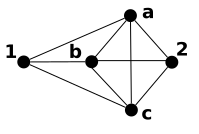
\includegraphics[width=3.5cm]{img/lemaClaw2Maximais} & &
    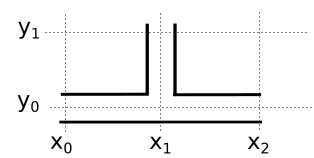
\includegraphics[width=5.5cm]{img/claw2}
    \\
    \footnotesize %\centering 
    (a)  \footnotesize Example of two maximal cliques sharing vertices. && \footnotesize (b) Representation  of a claw-clique in grid.\\
  \end{tabular}

 \caption{Vertices represented by a claw are present in a unique maximal clique.} \label{fig:lemaClaw2Maximais}
\end{figure}

% \begin{figure}[ht]
%   \centering
%   \begin{tabular}{  p{5cm} p{0.7cm} p{5cm} }
%     %\centering
%     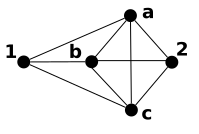
\includegraphics[width=3.5cm]{img/lemaClaw2Maximais} & &
%     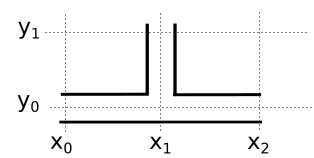
\includegraphics[width=5.5cm]{img/claw2}
%     \\
%     \footnotesize %\centering 
%     (a)  \footnotesize Examplo de duas cliques maximais compartilhando vértices. && \footnotesize (b) Representação de uma clique-garra na grade.\\
%   \end{tabular}

%  \caption{Vértices representados por uma garra  estão presentes em uma única clique maximal.} \label{fig:lemaClaw2Maximais}
% \end{figure}